\documentclass{beamer}
\usetheme{metropolis} % Use metropolis theme

\title{ECON 3818: Introduction to Statistics with Computer Applications}
%\subtitle
\date{\today}
\author{Kyle Butts}

\definecolor{blue}{RGB}{0,114,178}
\definecolor{red}{HTML}{EB0E09}
\definecolor{yellow}{RGB}{240,228,66}
\definecolor{green}{RGB}{0,158,115}
\definecolor{maroon}{HTML}{AF3335}
\definecolor{purple}{HTML}{7E90B8}
\definecolor{buff-gold}{HTML}{CFB87C}
\definecolor{buff-grey}{HTML}{565A5C}
\definecolor{buff-lightgrey}{HTML}{A2A4A3}
\definecolor{buff-black}{HTML}{000000}

\definecolor{mybackground}{HTML}{ECECEC}
\setbeamercolor{background canvas}{bg= mybackground}
\setbeamercolor{alerted text}{fg=buff-gold!80!black}
\setbeamercolor{frametitle}{bg=buff-black}
\setbeamercolor{title}{fg=buff-grey}
\setbeamercolor{button}{bg=buff-gold}

% Allow to remove indent w/ \begin{itemize}[leftmargin= *]
\usepackage{enumitem}
\setlist[itemize]{label= \textbullet}

% \usepackage[libertine]{newtxmath}
\usepackage{longtable}
\usepackage{booktabs}
\usepackage{enumitem}


\begin{document}

% Title Page ---------------------------------------
\maketitle




% Chapter 5 ----------------------------------------
\section{Chapter 5: Regression}

\begin{frame}{Review from Last Class}	
	Recall the ways we discussed relationships between two random variables $X$ and $Y$:
	\begin{itemize}
		
		\item Covariance, $\sigma_{XY}$ ($s_{XY}$)
		      \begin{itemize}
		      	\item Direction matters, but magnitude is hard to interpret
		      \end{itemize}
		      
		\item Correlation, $\rho_{XY}$ ($r_{XY}$)
		      \begin{itemize}
		      	\item Direction and magnitude matter
		      	\item Correlation is always value between $[-1,1]$
		      \end{itemize}
	\end{itemize}
	
\end{frame}

\begin{frame}{Review from Last Class}
	
	Recall: 
	$$r=\frac{cov(X,Y)}{\sqrt{V(X)}\cdot \sqrt{V(Y)}}$$
	
	\begin{itemize}
		\item Correlation is a function of covariance, just normalizes the magnitudes so we can interpret.
	\end{itemize}
	
\end{frame}

\begin{frame}{Clicker Question}
	
	Suppose you calculate the sample covariance, $s_{XY}=1.2$, and the sample standard deviations $s_X=2$ and $s_Y=2.5$. What is the sample correlation, $r_{XY}$?
	
	\begin{enumerate}[label=(\alph*)]
		\item 0.0576
		\item 0.24 %%
		\item 0.048
		\item 4.17
	\end{enumerate}
	
\end{frame}

\begin{frame}{Relationship between X and Y}
	
	We often summarize the relationship between $X$ and $Y$ using a straight line:
	\begin{center}
		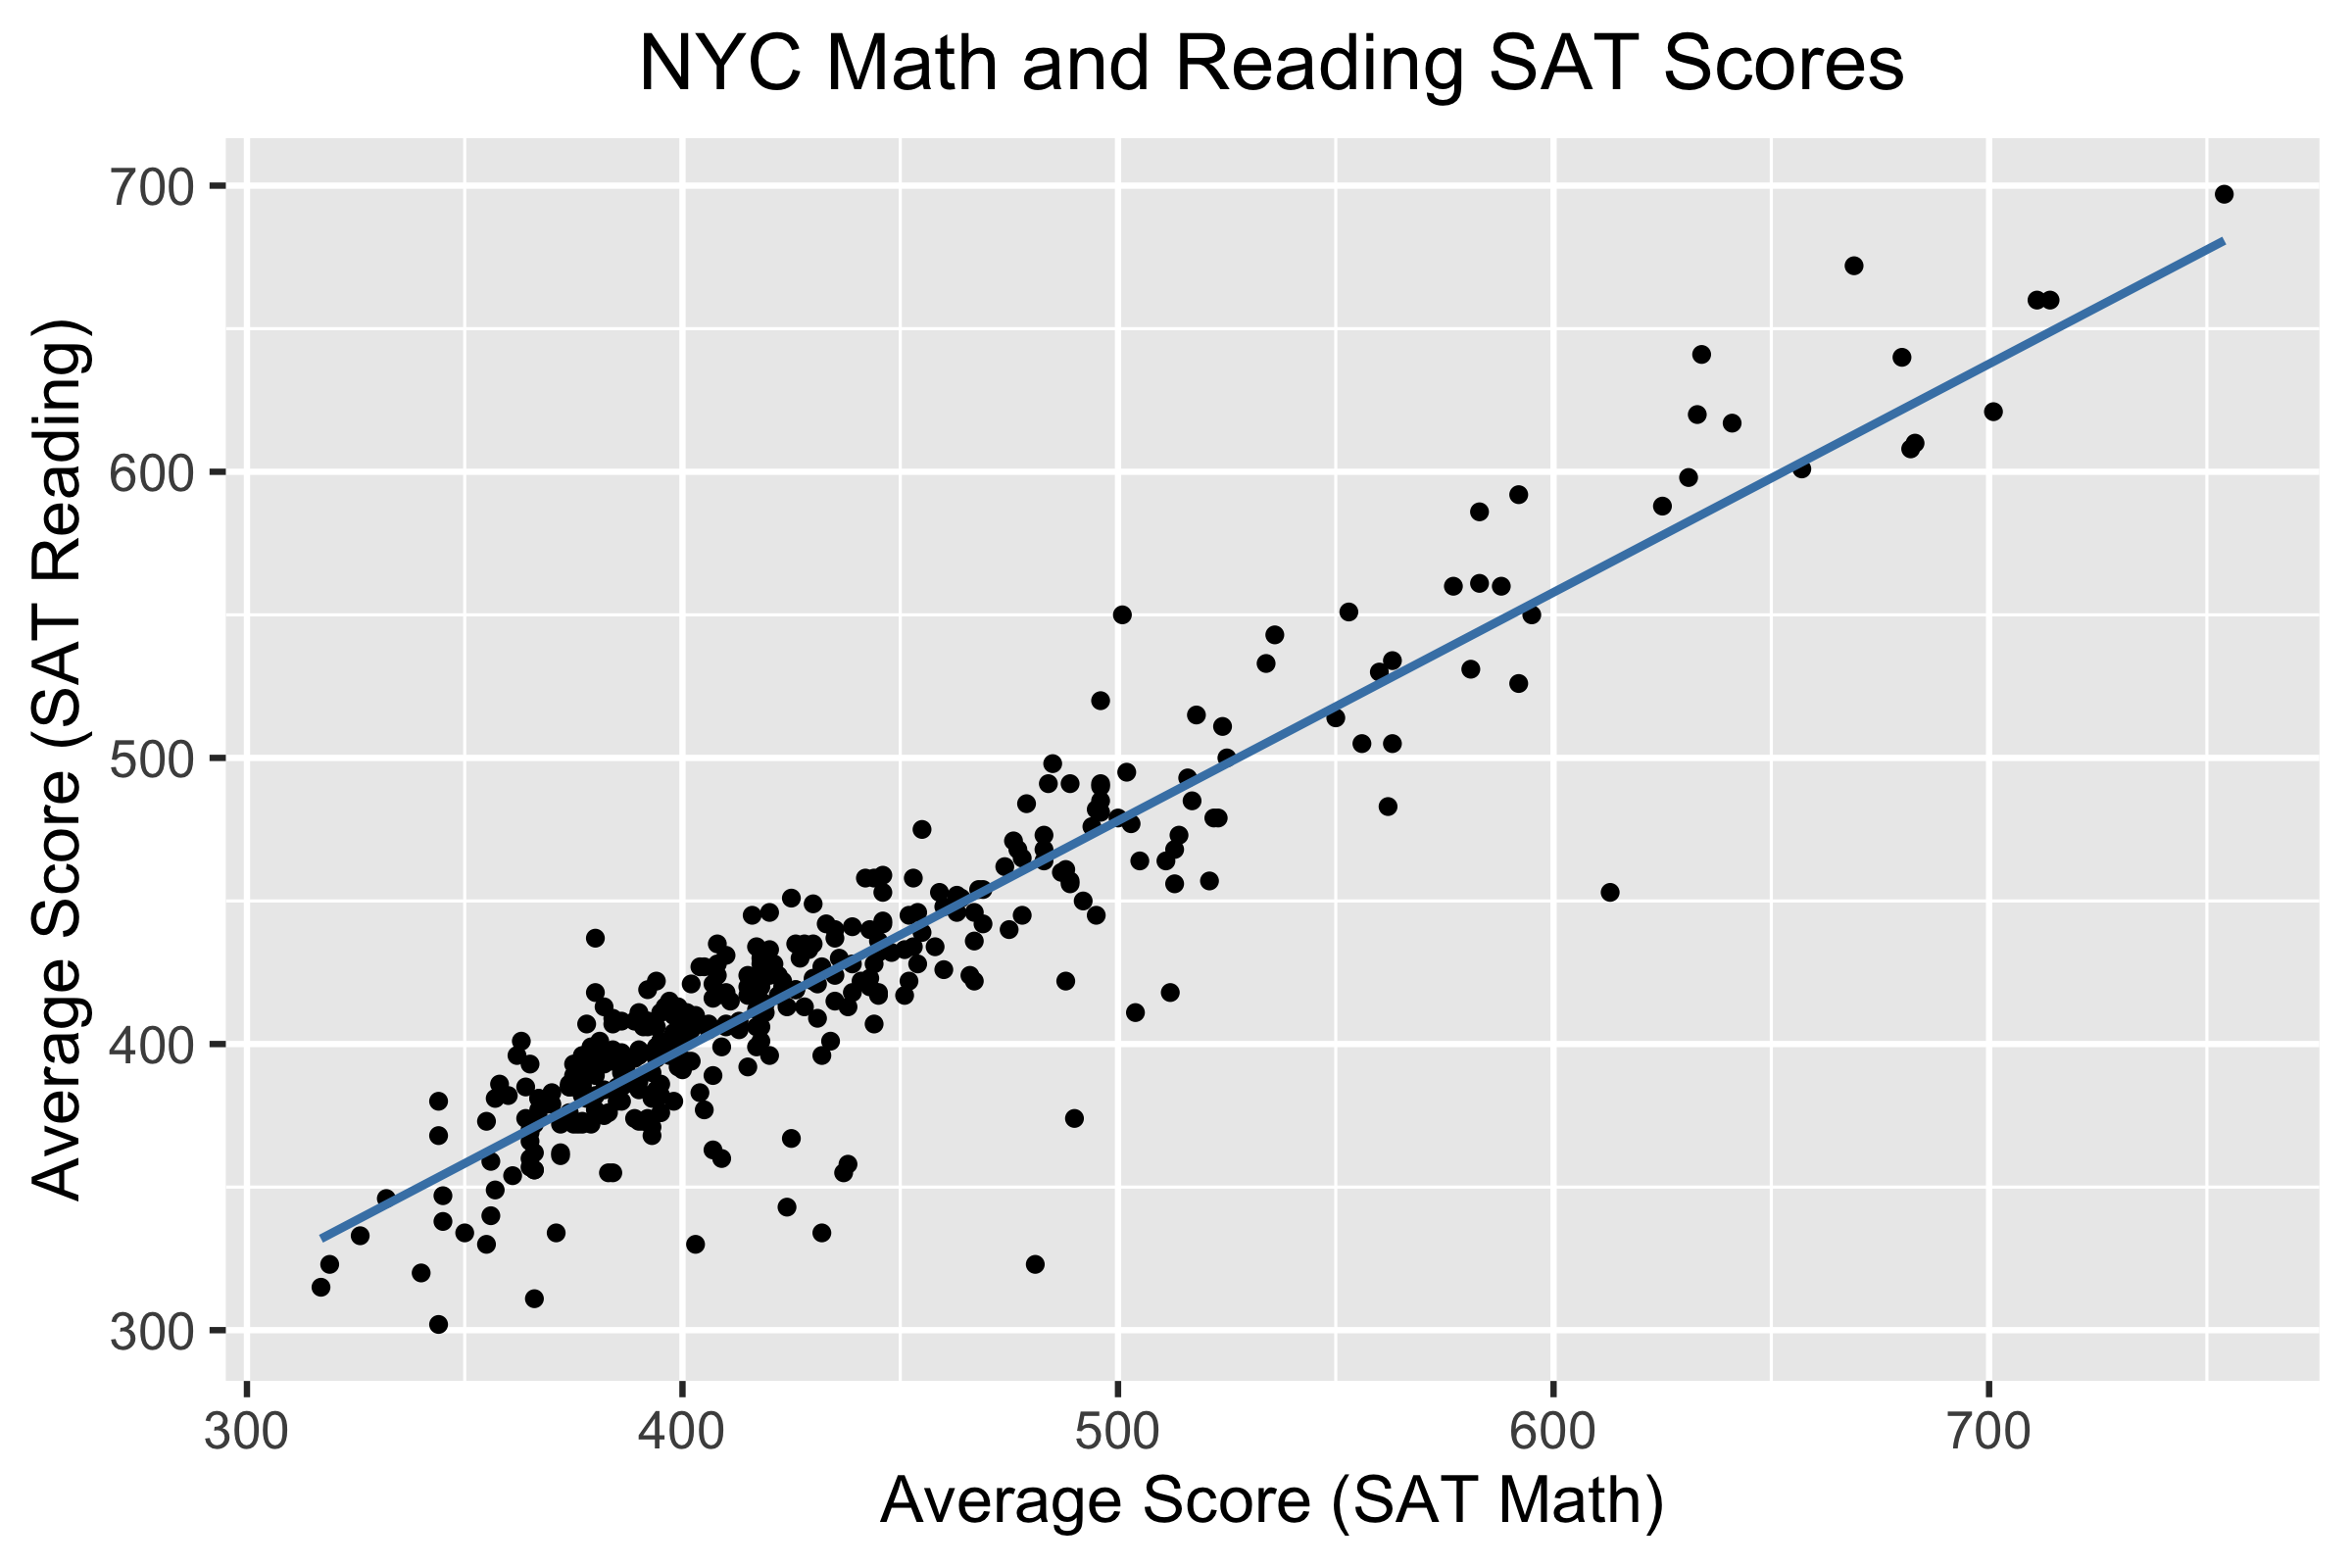
\includegraphics[width=.8\textwidth]{reg_line.png}
	\end{center}
	This is called the line of best fit, or the \alert{regression line}.
	
\end{frame}

\begin{frame}{Regression Line}
	\begin{definition}[Regression Line]
		Let $X$ and $Y$ be two random variables. A \alert{regression line} is a straight line that describes how the response variable, $Y$, changes as the explanatory variable $X$ changes.
	\end{definition}
	We often use a regression line to predict the value of $Y$ for a given value of $X$, \textit{when we believe the relationship between $X$ and $Y$ is linear.} 
	
	Assuming the relationship is actually linear, how do we find this line of ``best fit''?
\end{frame}
	
\begin{frame}{Least Squares Regression Line}
	What is the best straight line fit for the data? How would you determine it?
	\begin{center}
		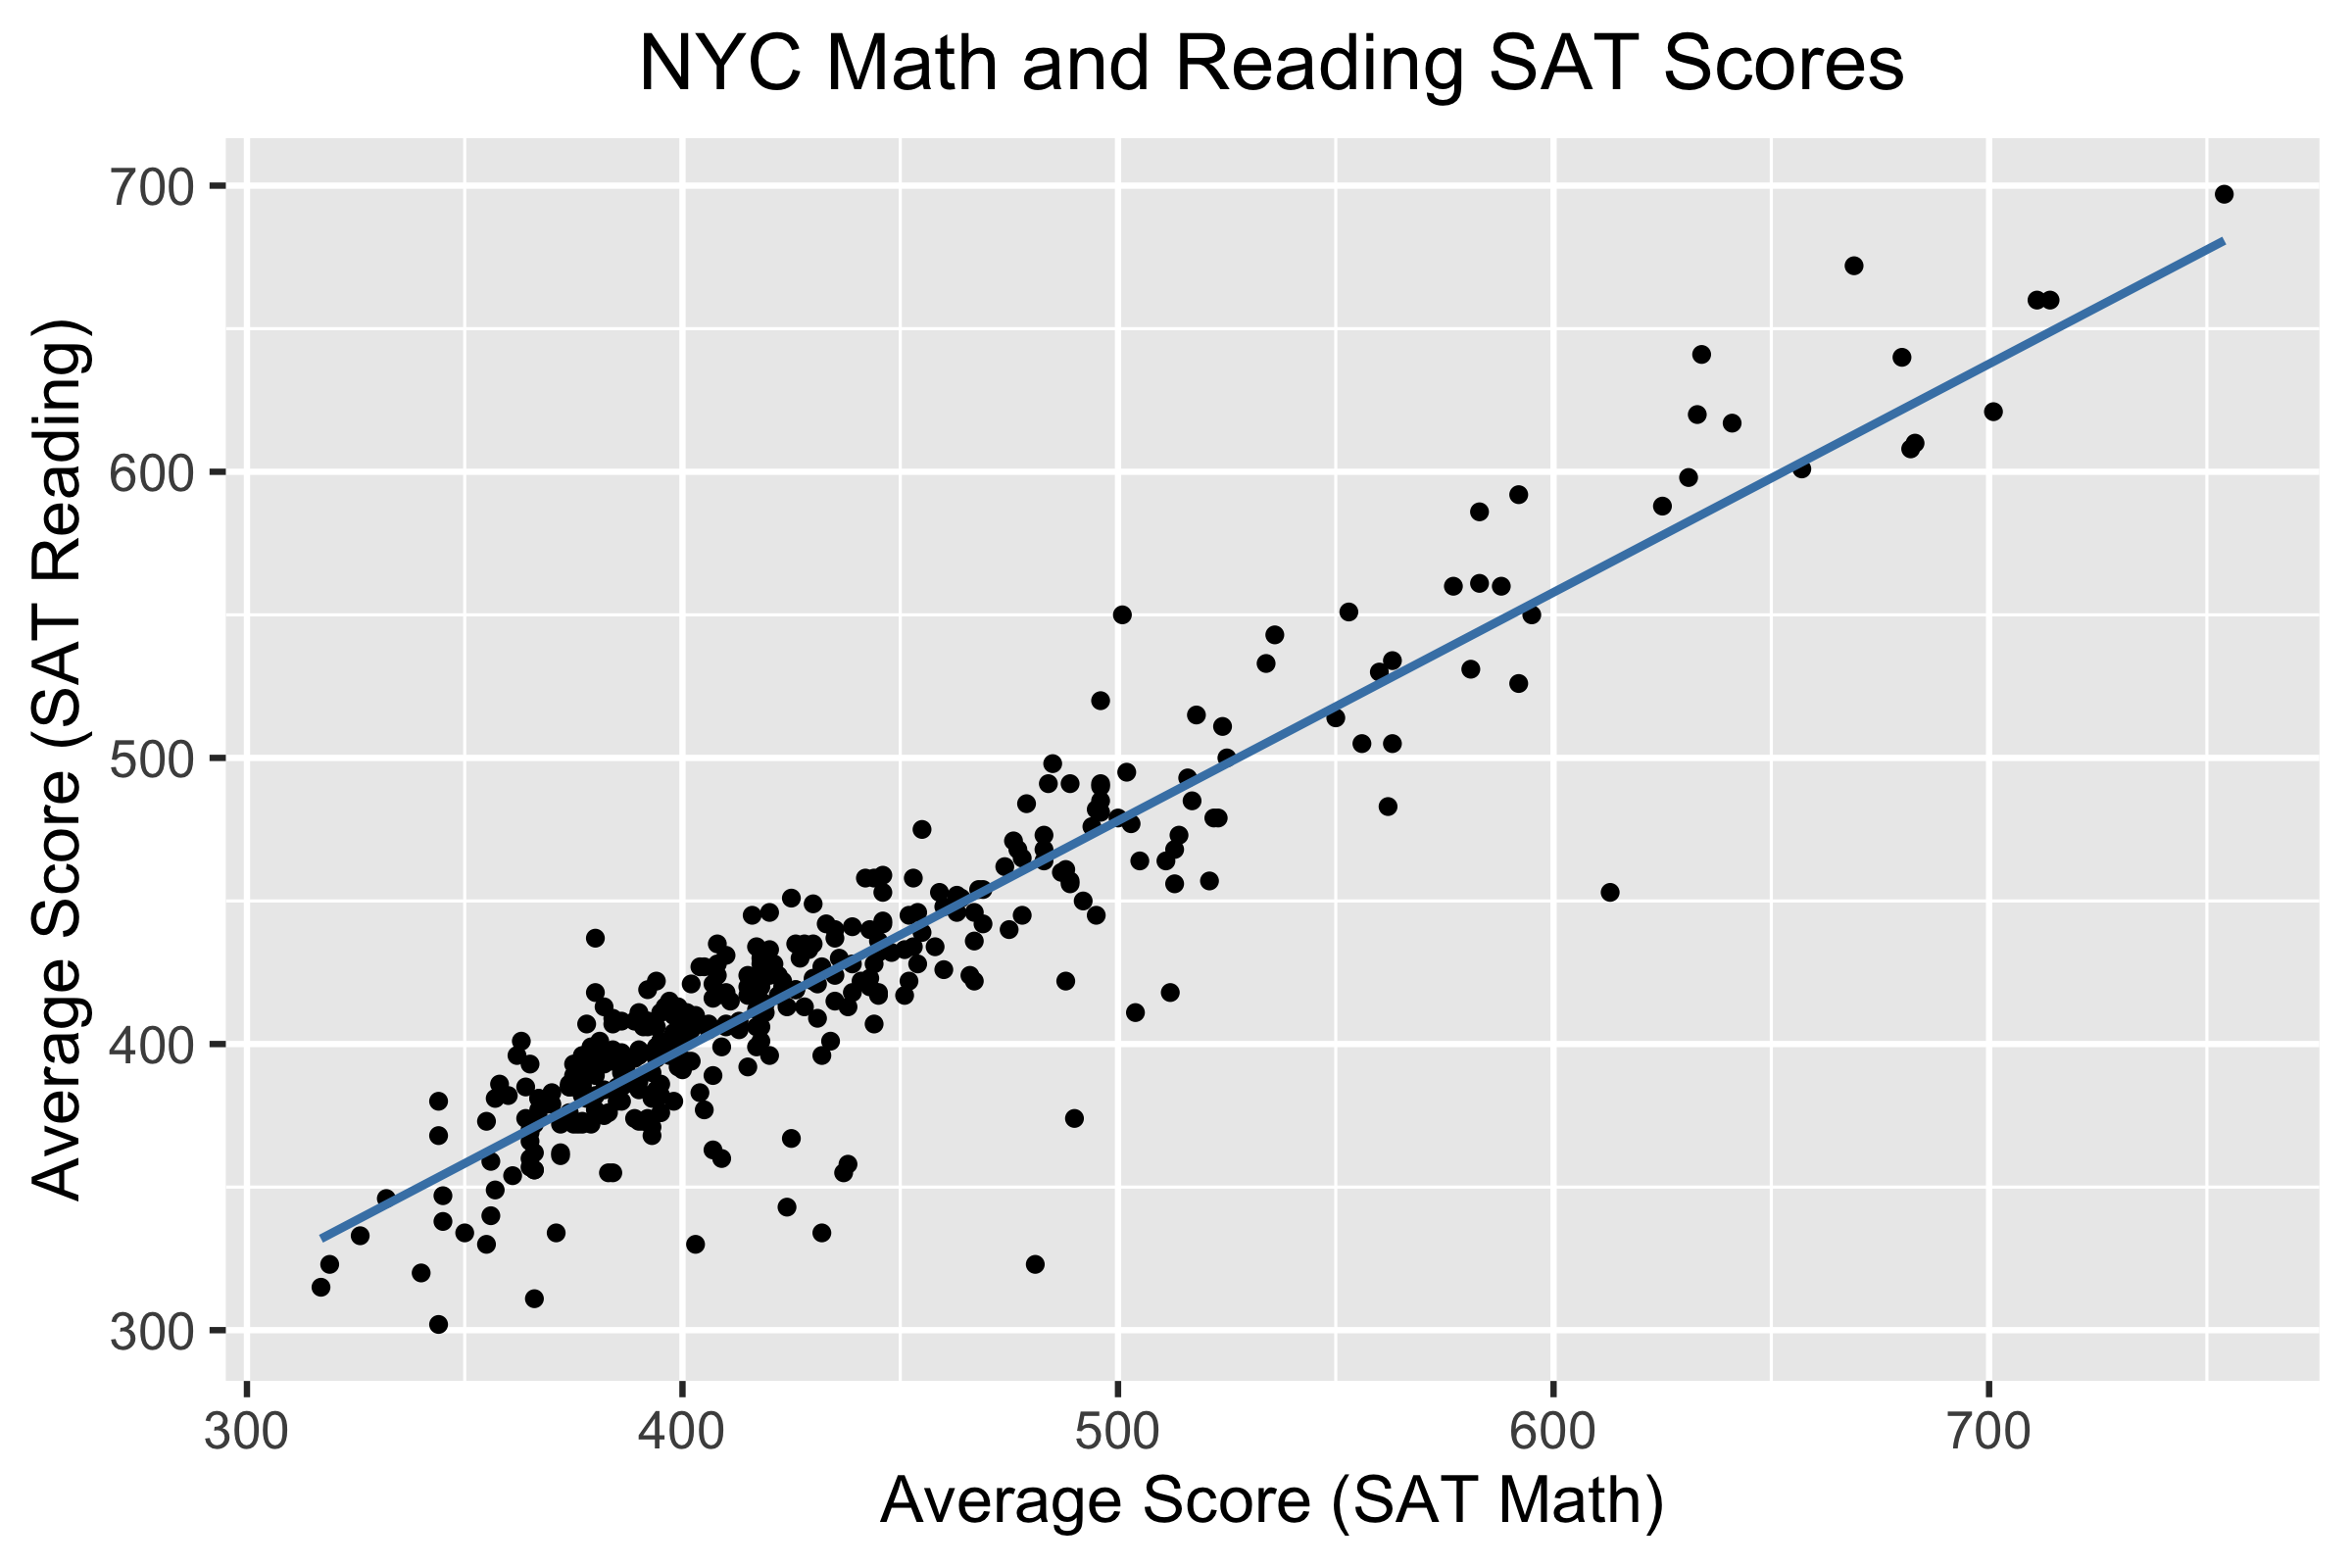
\includegraphics[width=.8\textwidth]{reg_line.png}
	\end{center}
\end{frame}

\begin{frame}{Least Squares Regression Line}
	What is the best straight line fit for the data? How would you determine it?
	\begin{center}
		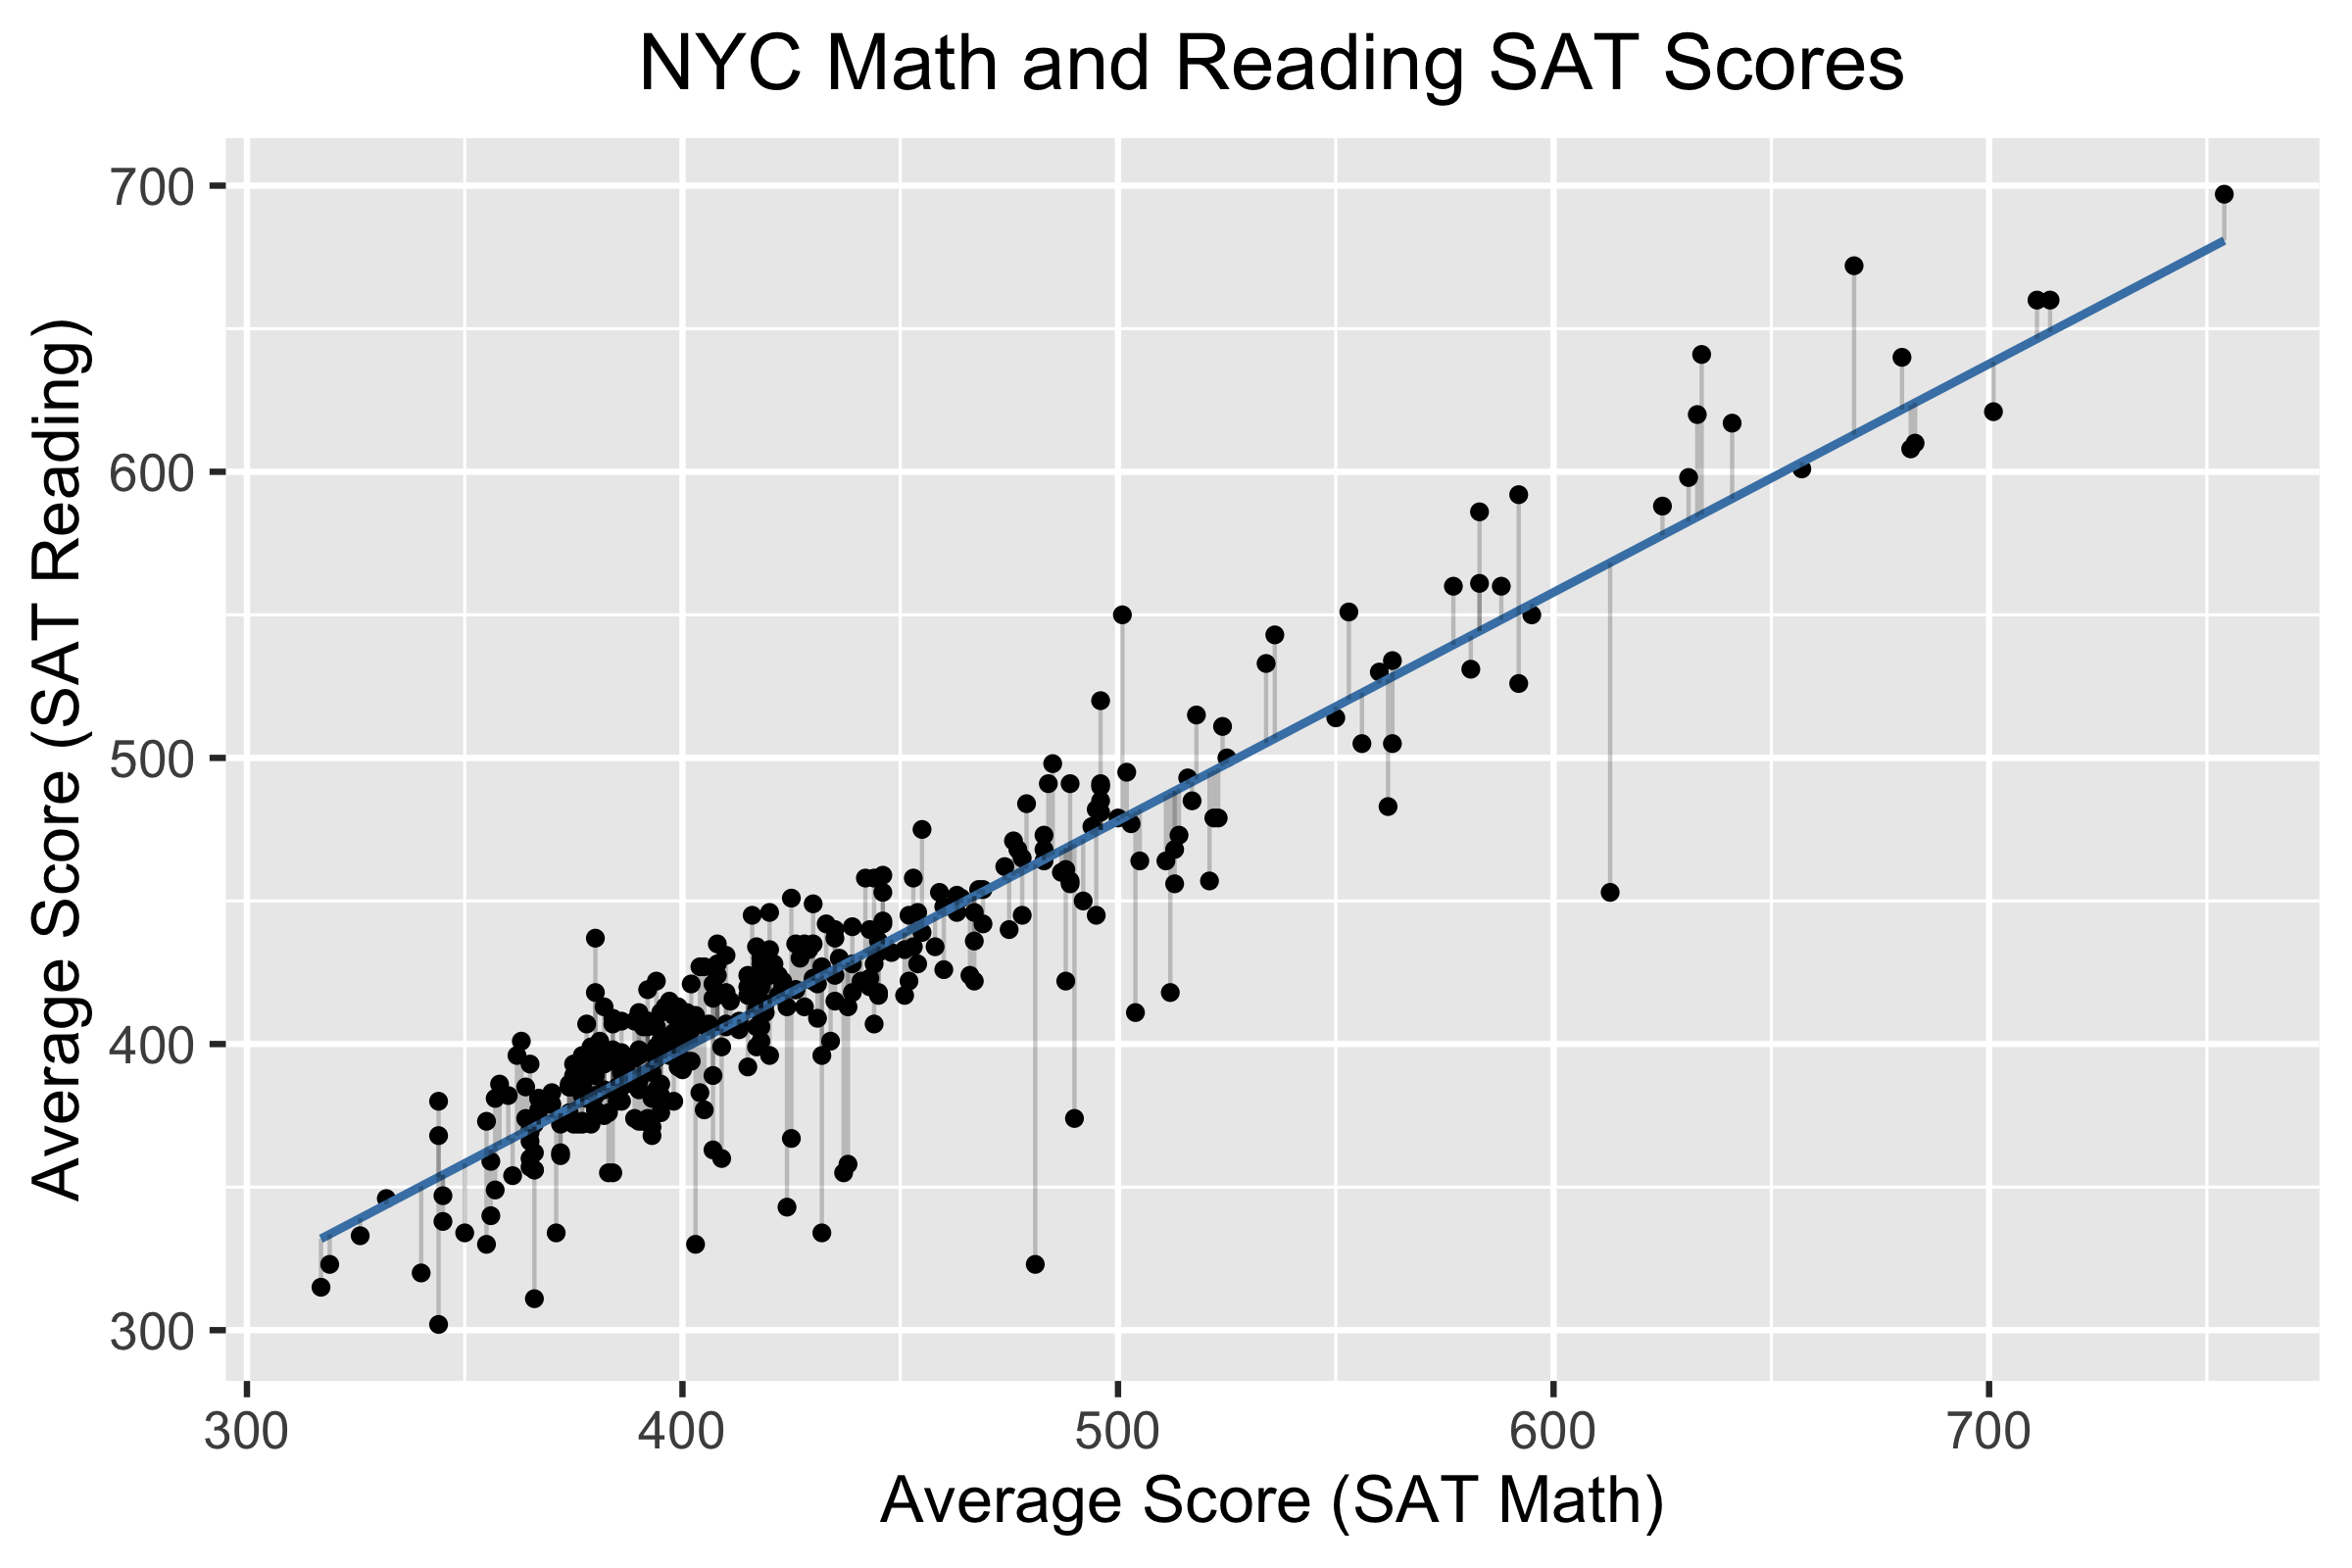
\includegraphics[width=.6\textwidth]{reg_line_resids.png}
	\end{center}
	We want to pick the line that minimizes the total error.
\end{frame}

\begin{frame}{Residual Error}
	Our goal is to pick a line that produces the least amount of total error. Let's define a \alert{residual} (error) as the difference between what we observe $(Y_i)$ and what we predict $(\hat{Y}_i)$:
	\[ \varepsilon_i = Y_i - \widehat{Y}_i. \]
	
	We could overestimate or underestimate, so $\varepsilon_i$ could be positive or negative. If we add up all the residuals, the positive and negatives will sometimes cancel.

	Therefore we want to minimize $\varepsilon_i^2$. Minimizing will produce $\varepsilon_i^2$ as close to 0 as possible.
	\vspace{.25in}
			
	We call $\displaystyle\sum_{i=1}^n \varepsilon_i^2 = \sum_{i=1}^n \left(Y_i - \widehat{Y}_i\right)^2$ the \alert{sum of squared residuals}.
\end{frame}

\begin{frame}{Least Squares Regression Line}
	Let's strictly define the least squares regression line.
	\begin{definition}[Least Squares]
		Let $\{X_i,Y_i\}_{i=1}^n$ be a random sample of $X$ and $Y$. The \alert{least squares regression line} is the equation $\widehat{Y}_i = a + bX_i$, where $a$ and $b$ solve
		\[ \min_{a,b} \sum_{i=1}^{n}\left( Y_i - \widehat{Y}_i \right)^2 = \sum_{i=1}^{n}\Big ( Y_i - \left(a+bX_i\right) \Big )^2 . \]
		The solution is $b=r_{XY}\frac{s_Y}{s_X}$ and $a = \bar{Y} - b\bar{X}$.
	\end{definition}
	
	We call $\widehat{Y}_i$ the \alert{predicted value} of $Y_i$ given $X_i$.
\end{frame}

\begin{frame}{Example}
	The least squares regression line for midterm grades is
	\[ \widehat{\text{SAT Reading}} = 78.87 + 0.7983 \cdot \text{SAT Math} \] 
	\begin{center}
		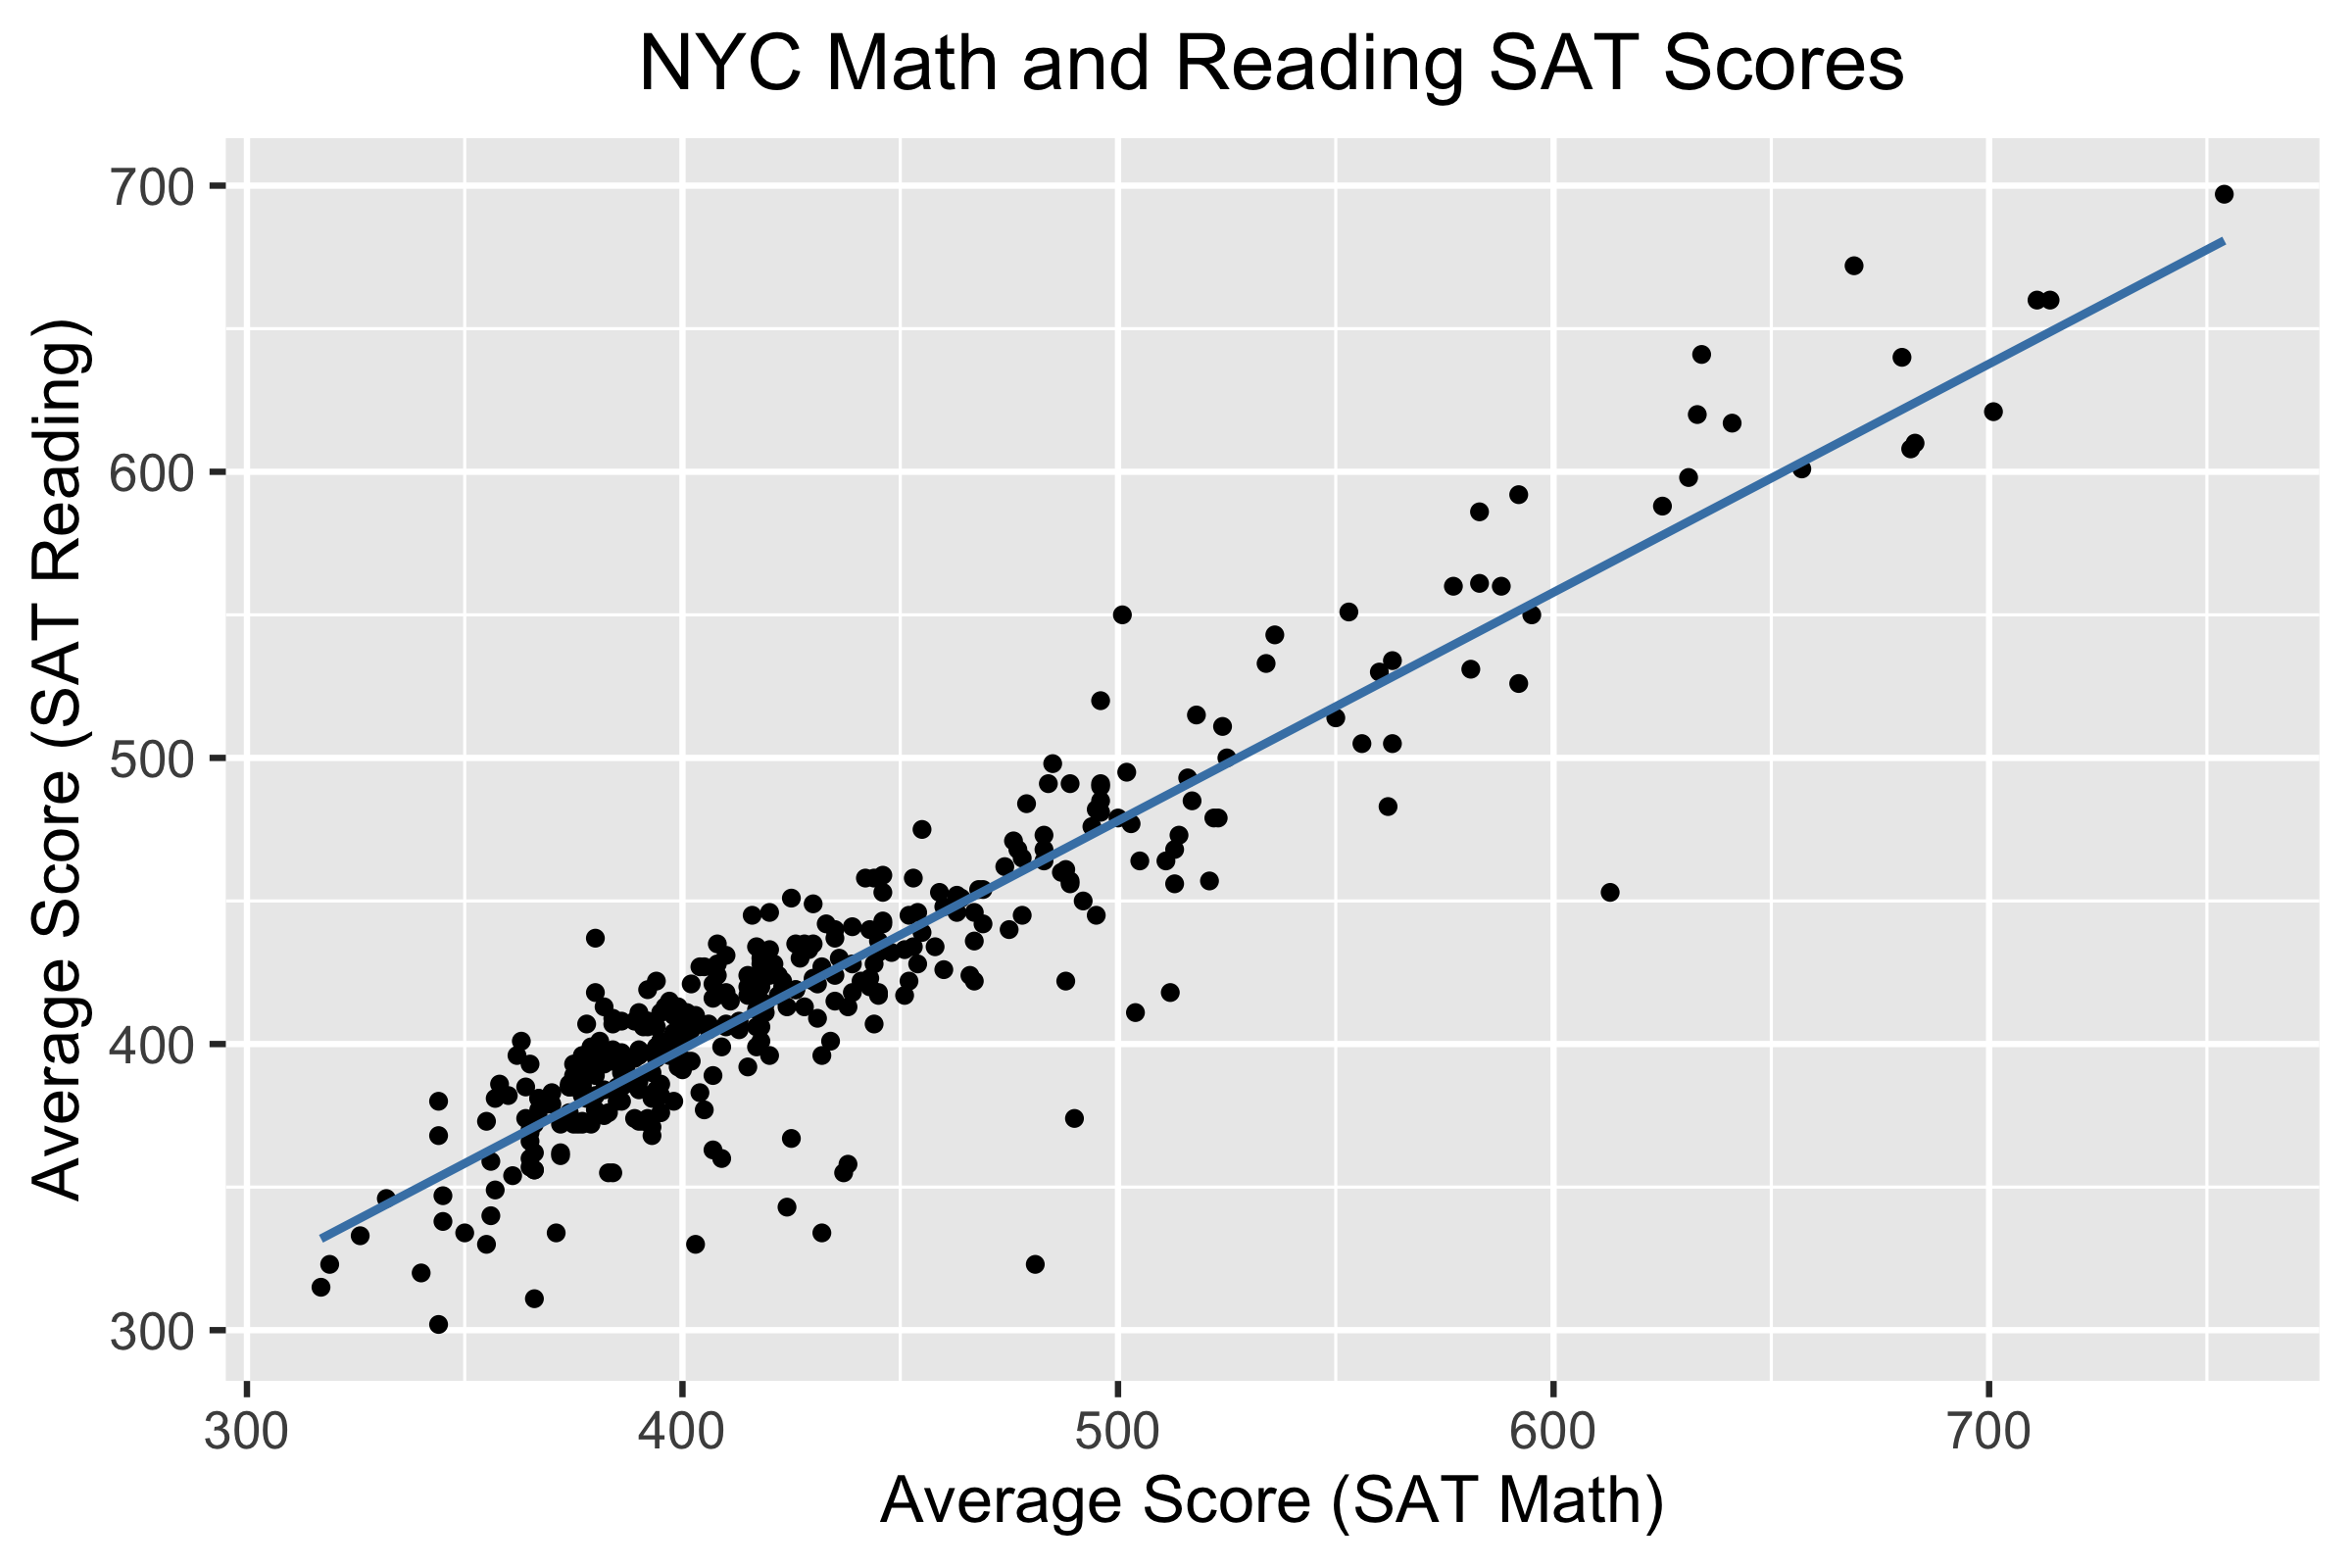
\includegraphics[width=.8\textwidth]{reg_line.png}
	\end{center}
\end{frame}

\begin{frame}{Takeaways of Least Squares Regression}
	
	\begin{itemize}
		\item Calculate regression by minimizing difference between predicted values and actual values
		      
		\item This leads to the following coefficients:
		      \begin{itemize}
		      	\item $b=r_{XY} \cdot \frac{s_Y}{s_X}$, the slope
		      	\item $a=\bar{Y}-b\bar{X}$, the intercept
		      \end{itemize}
	\end{itemize}
	
\end{frame}
	
\begin{frame}{Clicker Question}
	Consider the NHIS dataset. Let $Y$ be a person's weight in pounds, and $X$ be the number of drinks per day they consume (on average). You calculate the following:  
	\begin{align*} 
		\bar{Y} & =176.5889, \bar{X}=2.2489,                \\
		s_Y     & =39.86577, s_X=1.804856, r_{XY}=0.1187268 
	\end{align*}
	What is the regression line you fit to the data?
	\begin{enumerate}[label=(\alph*)]
		\item $\widehat{Y}_i=176.5889+2.6224X_i$
		\item $\widehat{Y}_i=176.5768+0.0054X_i$
		\item $\widehat{Y}_i=126.9151+22.08814X_i$
		\item {$\widehat{Y}_i=170.6913+2.6224X_i$} %%
	\end{enumerate}
\end{frame}
	
\begin{frame}{Regression Intuition}
	A regression line is a straight line that describes how a response variable $y$ changes as an explanatory variable $x$ changes
	
	We often use a regression line to predict the value of $y$ for a given value of $x$, when we believe the relationship is linear
	
	A linear relationship is of the form:
	$$y=a+b x$$
	so $a$ is the value of $y$ whenever $x=0$, and $b$ is the amount $y$ changes when $x$ increases by one
\end{frame}

\begin{frame}{Interpreting a Regression}
	Lets go back to our clicker question, we calculated the line of best fit to be:
	$$ \hat{Y}_i=170.69+2.62X_i$$
	where $Y$ is a person's weight in pounds, and $X$ is the number of drinks per day they consume (on average)
	
	\begin{itemize}
		\item Our intercept, 170.69 is the predicted weight for someone who doesn't consume any alcohol 
		      \begin{itemize} 
		      	\item The value of $\hat{Y}_i$ whenever $X_i$=0
		      \end{itemize}
		      
		\item Our slope, 2.62 is the amount predicted weight increases when number of drinks per day increases by 1
		      \begin{itemize}
		      	\item The amount $\hat{Y}_i$ changes when $X_i$ increases by 1
		      \end{itemize}
	\end{itemize}
\end{frame}

\frame

\begin{frame}{Interpreting a Regression}
	Say we calculate the following regression line from hours studied and final exam grades:
	$$\text{Final Exam}=38 + 5.7*\text{Hours of Studying}$$
	\begin{itemize}
		\item 38 is predicted score with no studying
		\item each hour of studying increases predicted final exam score by 5.7 points
	\end{itemize}
\end{frame}

\begin{frame}{Clicker Question}
	Given that same regression line, $\text{Final Exam}=38 + 5.7*\text{Hours of Studying}$, what is the predicted final exam score if you study 8 hours?
	
	\begin{enumerate}[label=(\alph*)]
		\item 83.6
		\item 45.6
		\item 96.3
	\end{enumerate}
\end{frame}

\begin{frame}{Clicker Question}
	A store in Boulder calculates a least squares line that describes how price (in dollars) of juuls affects the quantity sold; $$Juuls\text{ }sold = 117-12.4(price)$$ If price \textit{decreases} by 1 dollar, what happens to number of juuls sold?
	
	\begin{enumerate}[label=(\alph*)]
		\item Quantity decreases by 12.4
		\item Quantity increases 12.4
		\item Quantity decreases by 117
		\item Quantity increases by 117
	\end{enumerate}
\end{frame}

\begin{frame}{Properties of Regression Residuals}
	The slope, $b$, and intercept, $a$, of the regression line are found by minimizing $\sum_{i=1}^n \varepsilon_i^2$.
	\vspace{.25in}
			
	This forces $\bar{\varepsilon}=0$. Hence, an \alert{assumption} of regression is that $E(\varepsilon)=0$.
	\vspace{.25in}
			
	Intuitively, this assumption means that the error in your prediction is due entirely to randomness. 
\end{frame}

\begin{frame}{Overview of Regression Analysis}
	\small{A researcher is studying the relationship between high school students' SAT scores and their GPA during their freshman year of college. The data has a linear correlation coefficient of 0.503. Additional sample statistics are summarized in the table below:}
	
	\footnotesize{ \begin{tabular}{|c|c|c|c|}
		\hline 
		Variable & Description & Sample Mean & Sample Std. Dev \\ [0.5ex]
		\hline
		\rule{0pt}{15pt} X & SAT score & $\bar{X}=1501.72$ & $s_X=104.14$ \\ [0.5ex]
		\hline
		\rule{0pt}{15pt} Y & GPA & $\bar{Y}=3.3$ & $s_Y=0.45$ \\ [0.5ex]
		\hline
		\end{tabular}}
	
	\begin{itemize}
		\item What is the slope and intercept of this regression line? Write the linear regression using the $Y=a+bX$ format.
		\item Interpret the slope and intercept coefficients
		\item What is the predicted GPA if the student got a 1600 on the SAT?
	\end{itemize}
\end{frame}

	
\begin{frame}{$R^2$}
	Next we define a measure of goodness of fit.
	\begin{definition}[$R^2$]
		Let $\{X_i,Y_i\}_{i=1}^n$ be a random sample of $X$ and $Y$ and $\widehat{Y}_i$ be the predicted values. We define $R$-squared as
		\[ R^2 = \frac{\sum_{i=1}^n\left(\widehat{Y}_i - \bar{Y}\right)^2}{\sum_{i=1}^n\left(Y_i - \bar{Y}\right)^2} = r_{XY}^2, \]
		where $r_{XY}$ is the correlation coefficient for $X$ and $Y$.
	\end{definition}
\end{frame}
\begin{frame}{Intuition of $R^2$}
	
	Intuitively, $R^2$ measures the percent of variation in $Y$ explained by the model.
	$$r^2=\frac{\text{variation in } \hat{y} \text{ along the regression line as x varies}}{\text{total variation in observed values of y}}$$
	
\end{frame}
\begin{frame}{Visualizing $R^2$}
	\begin{center}
		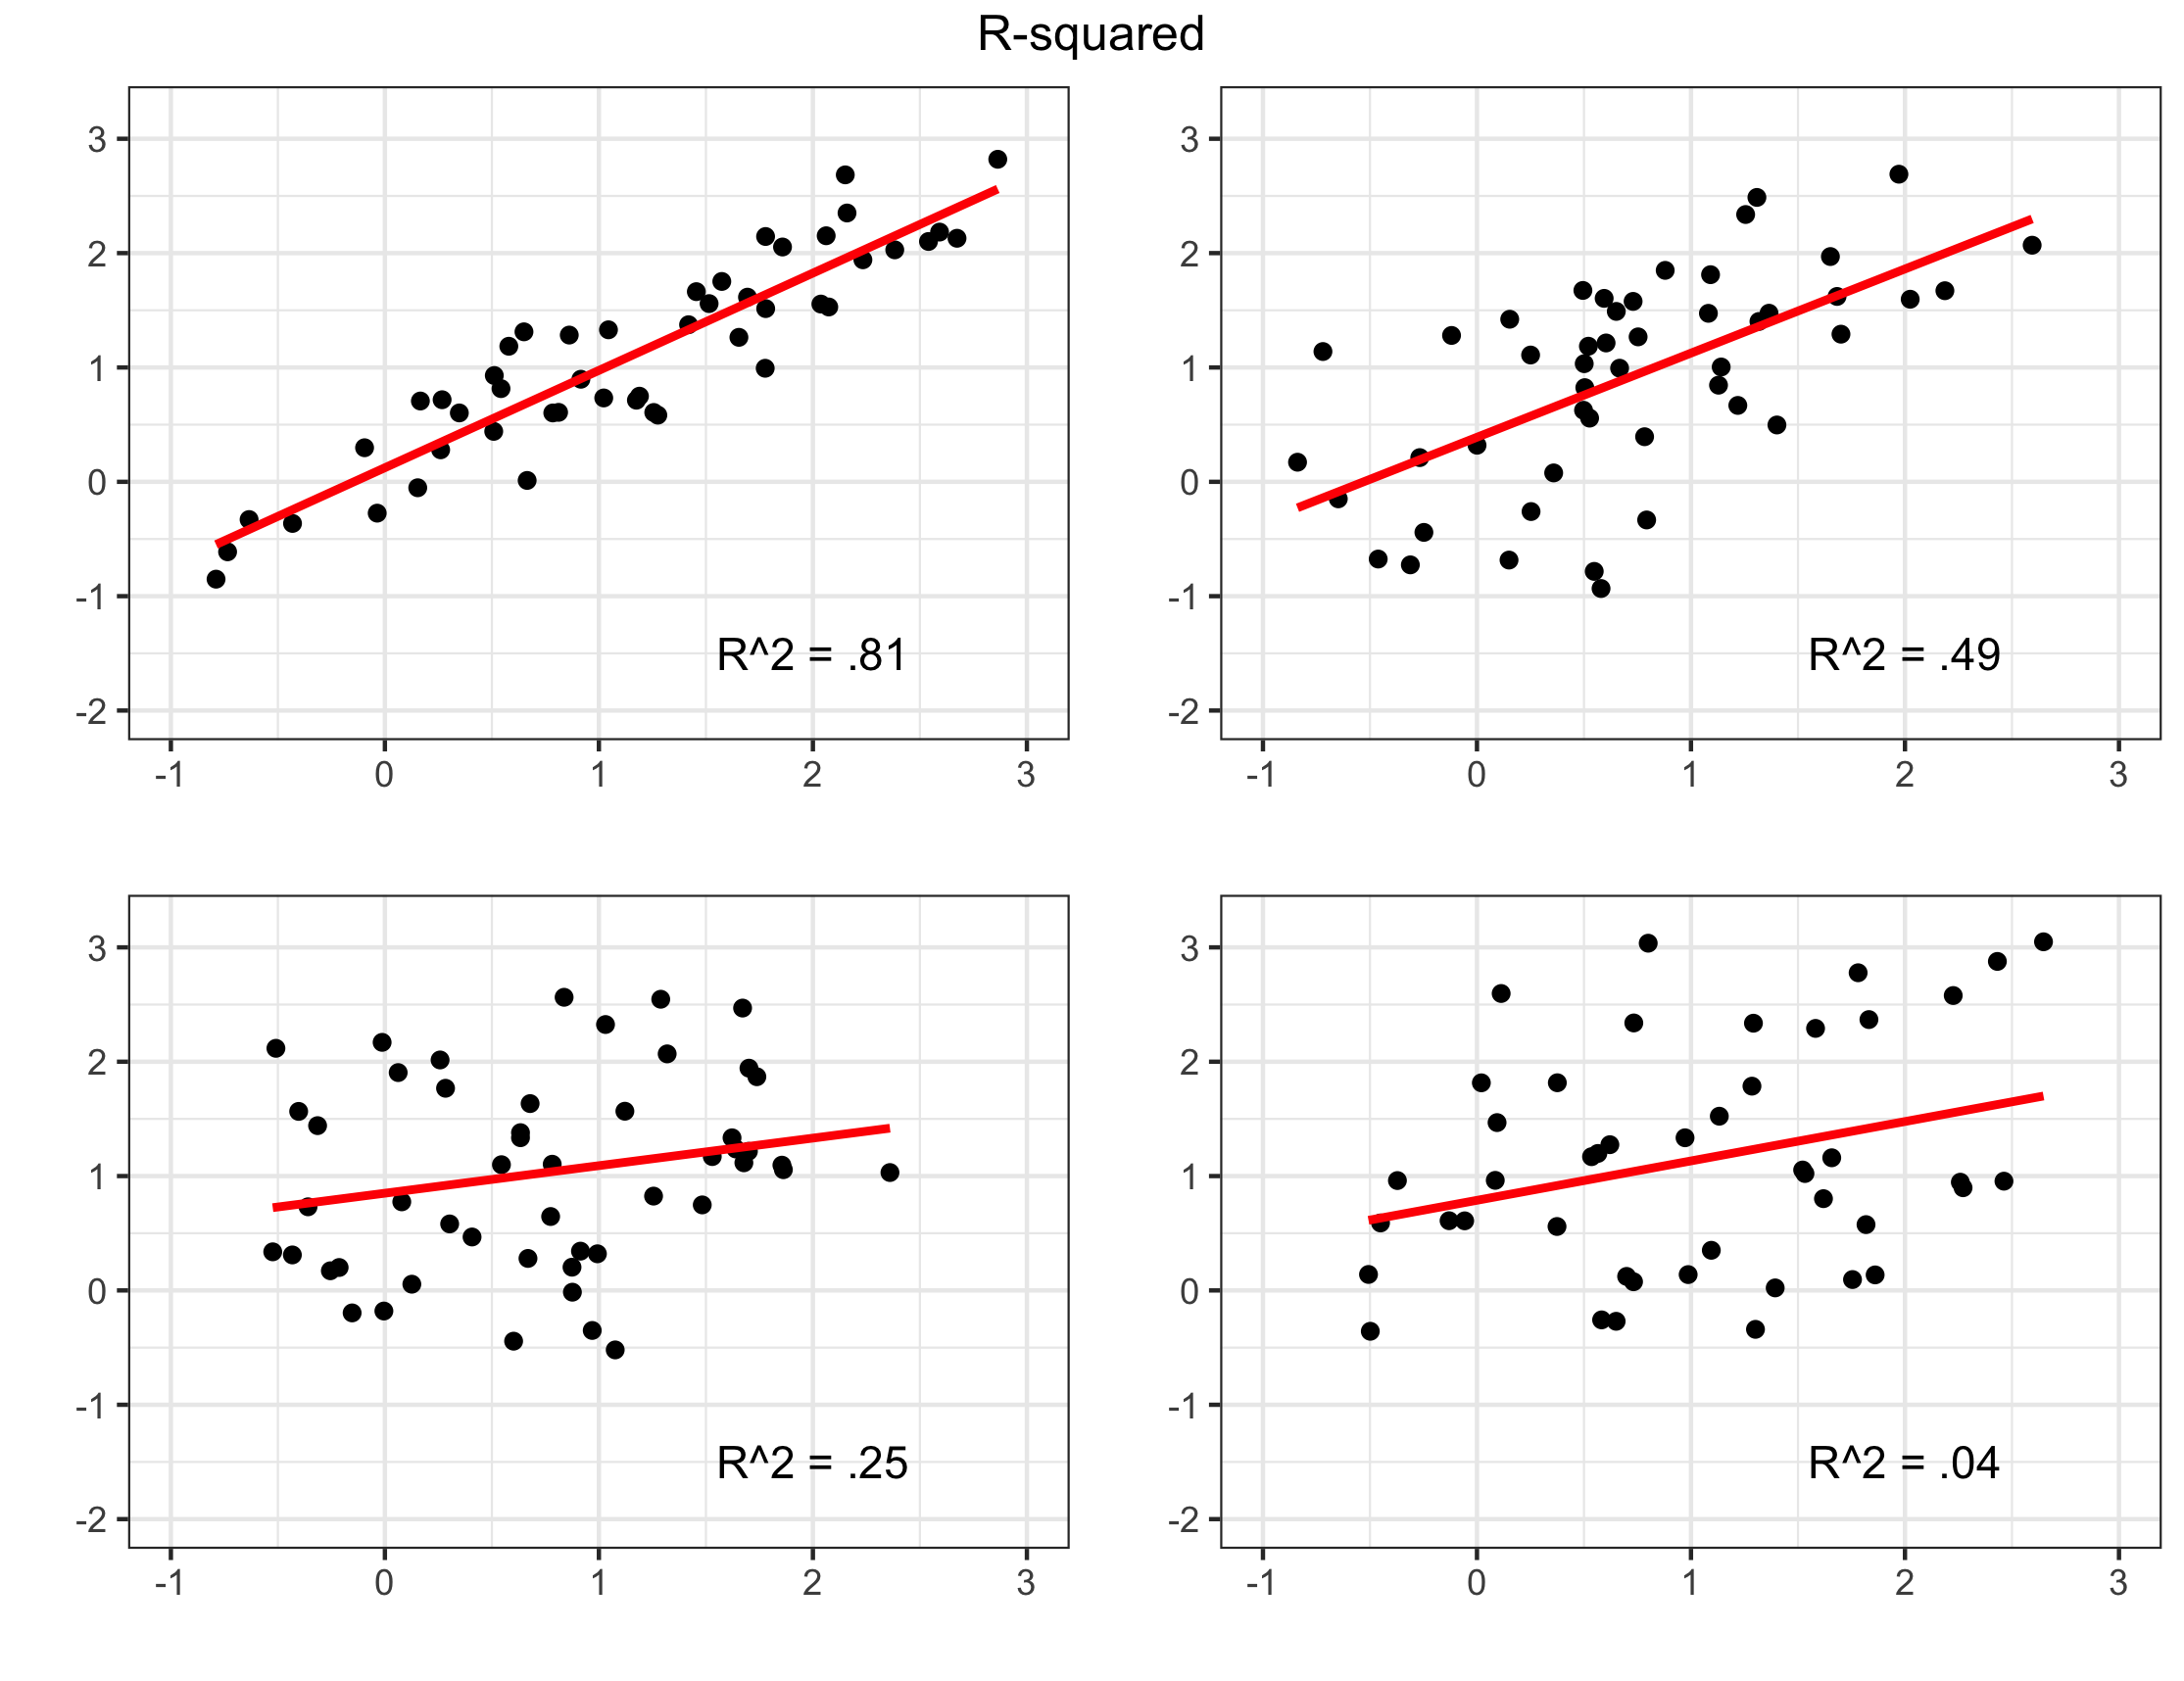
\includegraphics[width=.8\textwidth]{Rsquaredcomparisons.png}
	\end{center}
\end{frame}



\begin{frame}{$r$ and $R^2$}
	
	\begin{itemize}
		\item Correlation, $r$, describes the strength of a straight-line relationship between two variables
		      
		\item $R^2$, or $r^2$, is the fraction of the variation in the values of y that is explained by the least-squares regression of y on x
	\end{itemize}
	
\end{frame}

\begin{frame}{$r$ and $R^2$}
	
	Lets say we have $r=-0.7786$ and $r^2=(-0.7786)^2=0.6062$ between exercise and fat gain. 
	
	\begin{itemize}
		\item $r=-0.7786$, there is a strong negative linear relationship between time exercised and amount of weight gained
		\item $r^2=0.6062$, about 61\% of the variation in fat gained is accounted for by the linear relationship between fat gain and exercise. This means about 39\% of the change in fat gained is not explained by this relationship
	\end{itemize}
	
\end{frame}

\begin{frame}{Clicker Question}
	Say we run a regression on the temperature and the amount of gas used to heat a home. We fine that the $r=-0.99$ and $R^2=0.98$. This suggests that:
	
	\begin{enumerate}[label=(\alph*)]
		\item although temperature and gas used are very correlated, the temperature does not make very good predicts of the amount of gas used
		\item gas used increases by 0.99 cubic feet for each additional degree colder it is outside 
		\item prediction of gas used based off temperature will be quite accurate
	\end{enumerate}
\end{frame}

\begin{frame}{$R^2$ Sidebar}
	
	A small $R^2$ does not mean the result is uninteresting. All it means is that the x variable alone does not explain a large portion of the variation in y.
	
	Example: You find significant relationship between exercise and income, but it has a small $R^2$. We know income is determined by a variety of variables -- parent's income, education, innate ability, experience, etc. Your result isn't uninteresting, it just means there is a lot of variation in income \textit{not due} to exercise, which is exactly what we'd expect.
	
\end{frame}

\begin{frame}{$R^2$ Example}
	Recall from our previous example that a researcher calculated a correlation coefficient 0.503 between SAT scores and college freshman GPA. 
	
	This implies an $R^2$ of 0.253. 
	
	What does this $R^2$ mean? Does this make sense, what other things could explain the variation in freshman year GPA?
\end{frame}


\begin{frame}{Influential Observations}
	
	Our regression line is sensitive to outliers, either in the x or y dimension 
	\begin{itemize} 
		\item We say an outlier is \alert{influential} if deleting it changes our regression line substantially
		\item The amount by which the line changes is called the \alert{leverage} an influential observation has
	\end{itemize}
	
\end{frame}

\begin{frame}{Influential Observations}
	Suppose we had an outlier of a Math score of 700 and a Reading score of 340. That data point has quite a bit of leverage because it is an extreme outlier.
	\begin{center}
		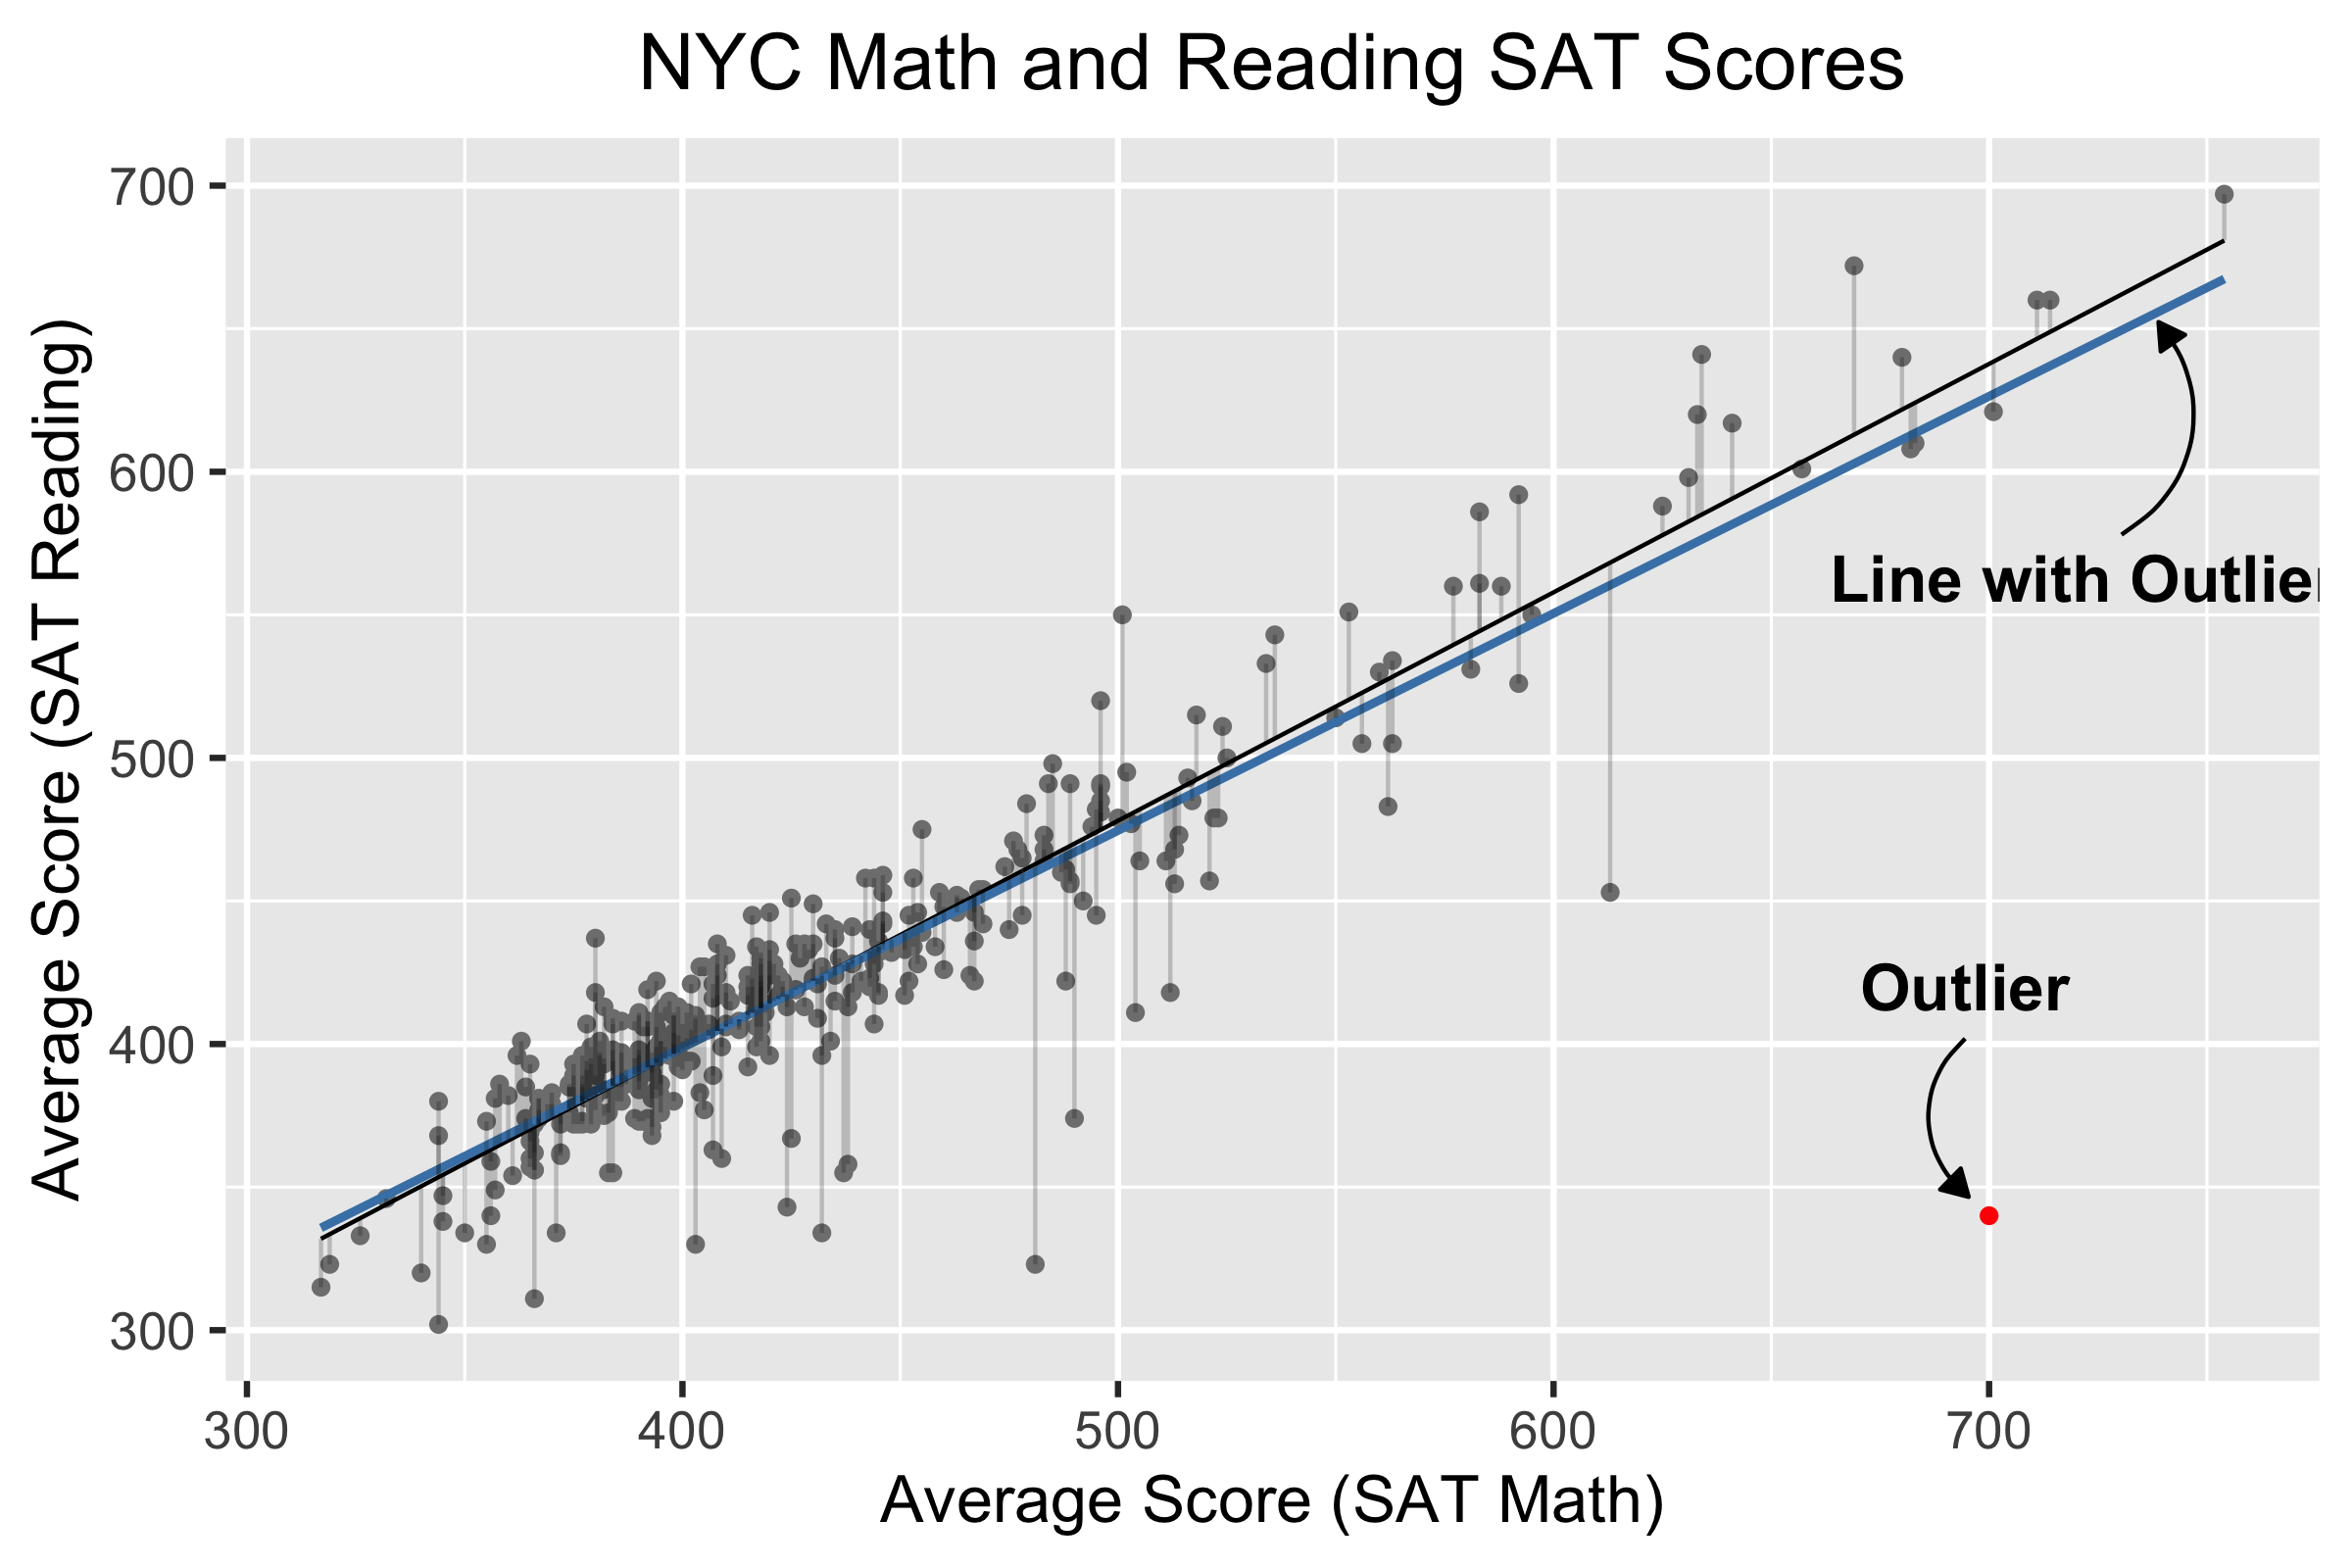
\includegraphics[width=0.9\textwidth]{influentialobs}
	\end{center}
\end{frame}

\begin{frame}{Cautions about Correlation and Regression}
	Correlation and regression are powerful tools for describing the relationship between two variables, but they have their limitations
	\begin{itemize}
		\item These tools only describe linear relationships
		\item They are not resistant to outliers 
	\end{itemize}
	Now we will introduce three other potential issues with these tools
	\begin{itemize}
		\item Ecological correlation
		\item Extrapolation
		\item Lurking variables
	\end{itemize}
\end{frame}

\begin{frame}{Ecological Correlation}
	
	A correlation based on averages rather than on individuals is called an \alert{ecological correlation}. The idea being that the correlation between averages may be stronger than the correlation at the individual level 
	
	Examples:
	\begin{itemize}
		\item Number of years of education and average income level
		\item Hours of weekly exercise and body mass index
	\end{itemize}
	
	These relationships are very strong when we look at everyone, but may not be as strong when we analyze at the individual level
	
\end{frame}

\begin{frame}{Extrapolation}
	
	\alert{Extrapolation} is the use of a regression line for a prediction far outside the range of values of the explanatory variable $x$ that you used to obtain the line
	
	The idea here is that not many relationships are linear for \textit{all values of x}
	
	Example:
	\begin{itemize}
		\item Age and height, eventually you stop growing 
		\item Experience and pay, eventually your salary levels off (usually)
	\end{itemize}
	
\end{frame}

\begin{frame}{Lurking Variable}
	
	A \alert{lurking variable} is a variable that is not among the explanatory or response in a study and yet may influence the interpretation of relationships among those variables. Also known as omitted variable bias.
	\begin{itemize}
		\item Experience in music and test scores -- family background is a lurking variable
		\item Ice cream sales and number of violent police reports -- both of these things increase when the weather is warm
	\end{itemize}
	
\end{frame}



\begin{frame}{Cautions about Correlation and Regression}
	With all these limitations and potential issues, it is important to remember:
	\begin{center}
		\Large{\alert{Correlation does not imply causation}}
	\end{center}
\end{frame}



\begin{frame}{Clicker Question}
	A study of elementary school children, ages 6 to 11, finds a high positive correlation between shoe size and score on a test of reading comprehension. The observed correlation is most likely due to:
	\begin{enumerate}[label=(\alph*)]
		\item cause and effect (larger shoe size causes higher reading comprehension)
		\item a mistake, because the correlation must be negative
		\item the effect of a lurking variable, such as age or years of reading experience
		\item reverse cause and effect (higher reading comprehension causes larger shoe size)
	\end{enumerate}
\end{frame}

\begin{frame}{Spurious Correlations}
	
	\begin{itemize}
		\item \alert{Spurious Correlation} is things move in the same direction, even if they are completely unrelated.
	\end{itemize}
	
	\begin{center}
		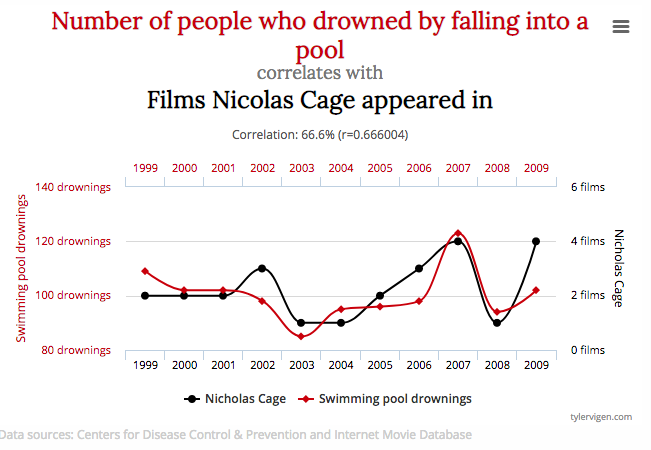
\includegraphics[width=\textwidth]{spcorr1}
	\end{center}
	{\footnotesize http://www.tylervigen.com/spurious-correlations}
	
\end{frame}

\begin{frame}{Spurious Correlations}
	\begin{center}
		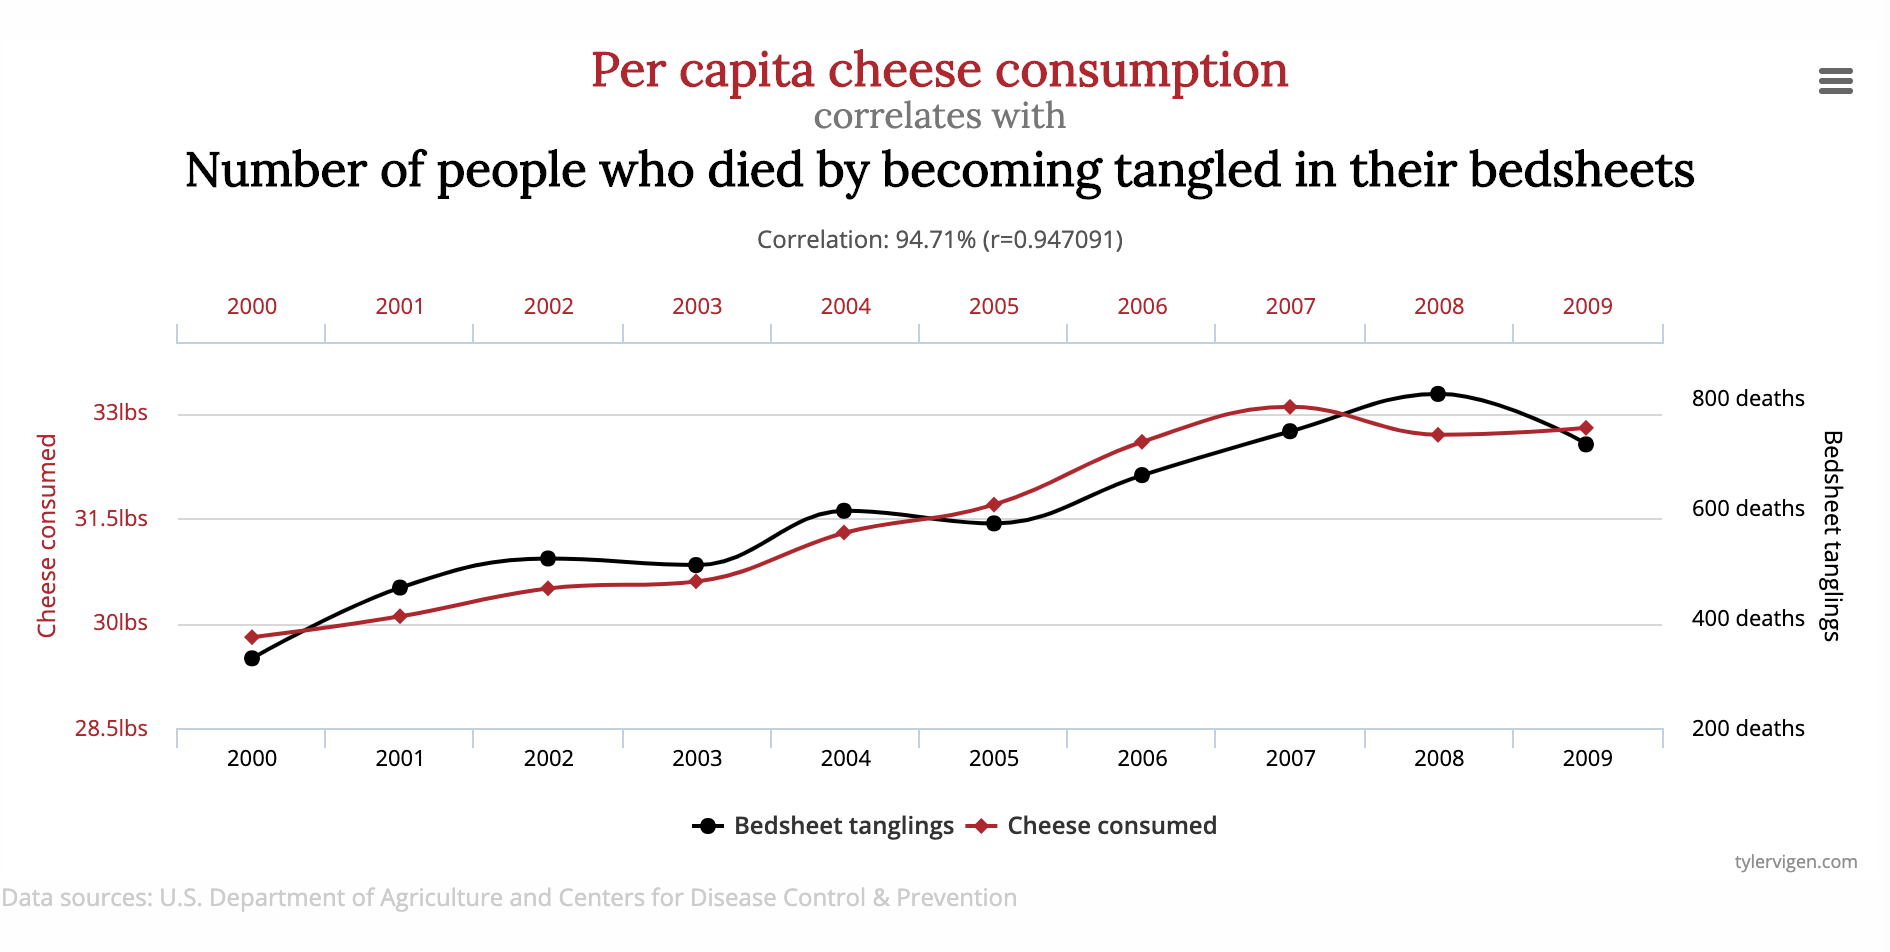
\includegraphics[width=\textwidth]{spurious2}
	\end{center}
\end{frame}


\end{document}